

% ****** Start of file aipsamp.tex ****m*
%
%   This file is part of the AIP files in the AIP distribution for REVTeX 4.
%   Version 4.1 of REVTeX, October 2009
%
%   Copyright (c) 2009 American Institute of Physics.
%
%   See the AIP README file for restrictions and more information.
%
% TeX'ing this file requires that you have AMS-LaTeX 2.0 installed
% as well as the rest of the prerequisites for REVTeX 4.1
% 
% It also requires running BibTeX. The commands are as follows:
%
%  1)  latex  aipsamp
%  2)  bibtex aipsamp
%  3)  latex  aipsamp
%  4)  latex  aipsamp
%
% Use this file as a source of example code for your aip document.
% Use the file aiptemplate.tex as a template for your document.
\documentclass[%
 aps, prl,
% jmp,
% bmf,
% sd,
% rsi,
 amsmath,amssymb,
%preprint,%
 reprint,%
%author-year,%
%author-numerical,%
% Conference Proceedings
superscriptaddress
]{revtex4-2}

\usepackage{graphicx}% Include figure files
%\usepackage{dcolumn}% Align table columns on decimal point
\usepackage{bm}% bold math
\usepackage{fixme}
%\usepackage[mathlines]{lineno}% Enable numbering of text and display math
%\linenumbers\relax % Commence numbering lines
\usepackage{hyperref}
\usepackage{kbordermatrix}% http://www.hss.caltech.edu/~kcb/TeX/kbordermatrix.sty
\usepackage[utf8]{inputenc}
\usepackage[T1]{fontenc}
\usepackage{mathptmx}
\usepackage{lipsum}
\usepackage{amsmath}
\usepackage{physics}
\usepackage{xparse}
\usepackage{bbm}
\usepackage{xcolor}
\usepackage{url}


%\usepackage{multirow}
%\usepackage{makecell}
\graphicspath{{Pictures/}}

\renewcommand*{\figureautorefname}{Fig.}
\renewcommand*{\equationautorefname}{Eq.}

\newcommand{\mytitile}{Photon transport and chaos in a Bose-Hubbard chain of superconducting artificial atoms}

\begin{document}
	\preprint{AIP/123-QED}
	
	\title[\mytitile]{\mytitile\\~}
	\author{G.P. Fedorov}
	\email{gleb.fedorov@phystech.edu}
	
	\affiliation{ 
		Russian Quantum Center, Skolkovo village, Russia
	}%
	\affiliation{ 
		Moscow Institute of Physics and Technology, Dolgoprundiy, Russia
	}
	\affiliation{
		National University of Science and Technology MISIS, Moscow, Russia
	}%

	\author{I.A. Rodionov}
	\affiliation{FMN Laboratory, Bauman Moscow 
	State Technical University, Moscow, Russia}
	\affiliation{Dukhov Automatics Research 
	Institute, (VNIIA), Moscow, Russia}
	
	
	\author{A.A. Dobronosova}
	\affiliation{FMN Laboratory, Bauman Moscow 
	State Technical University, Moscow, Russia}
	\affiliation{Dukhov Automatics Research 
	Institute, (VNIIA), Moscow, Russia}
	
	
	\author{D.O. Moskalev}
	\affiliation{FMN Laboratory, Bauman Moscow 
	State Technical University, Moscow, Russia}
	
	
	\author{A.A. Pishchimova}
	\affiliation{FMN Laboratory, Bauman Moscow 
	State Technical University, Moscow, Russia}
	\affiliation{Dukhov Automatics Research 
	Institute, (VNIIA), Moscow, Russia}
	
	\author{E.I. Malevannaya}
	\affiliation{FMN Laboratory, Bauman Moscow 
		State Technical University, Moscow, Russia}
	\affiliation{Dukhov Automatics Research 
		Institute, (VNIIA), Moscow, Russia}

	\author{O.V. Astafiev}
	\affiliation{Skolkovo Institute of Science 
		and Technology, Moscow, Russian Federation}
	\affiliation{ 
		Moscow Institute of Physics and Technology, 
		Dolgoprundiy, Russia
	}
	\affiliation{Physics Department, Royal 
	Holloway, University of London, Egham, Surrey 
	TW20 0EX, United Kingdom}
\affiliation{National Physical Laboratory, Teddington, TW11 0LW, United Kingdom}
%
	
	
	\date{\today}% It is always \today, today,
	%  but any date may be explicitly specified
	
	
	\begin{abstract}
We investigate non-equilibrium steady-state photon transport through a chain of five coupled artificial atoms described by the Bose-Hubbard model. By increasing incident photon flux, we demonstrate a continuous transition from the linear regime described by the classical coupled oscillators model to the quantum regime of photon blockade characterized by suppressed transmission and complex structure of multiphoton resonances. We show excellent agreement of the transmission with the input-output theory for a model with around a hundred basis states. Next, we demonstrate that our architecture allows straightforward and high-contrast visualization of the emergent energy bands via cross-Kerr spectroscopy. Finally, we show how controllable disorder in the system suppresses this non-local photon transmission. We argue that our architecture may be applied for analog simulation of many-body Floquet dynamics with even larger arrays of artificial atoms paving an alternative way to quantum supremacy.
	\end{abstract}
	
	\maketitle


There has been increased effort over recent years in analog simulation of various models from solid state physics and quantum optics on a chip using superconducting circuits \cite{kjaergaard2019superconducting}. The Bose-Hubbard (B-H) model is now particularly well-covered as it can be directly mapped onto arrays of coupled transmons \cite{orell2019probing}. The first work \cite{hacohen2015cooling} had demonstrated this for a three-site linear lattice, and subsequent experiments were focused either on simulating dynamics with engineered dissipation \cite{ma2019dissipatively}, or studying the many-body localization phase transitions \cite{roushan2017spectroscopic,chiaro2019growth}, or correlated quantum walks \cite{Yan2019, Ye2019}.

Numerous theoretical studies propose a new possible direction: controllable light-matter interaction and Floquet engineering to model periodically-driven Hamiltonians and their non-equilibrium dynamics \cite{Goldman2014, eisert2015quantum, Zippilli2015, kyriienko2018floquet, franca2020simulating}. Particularly, a recent study has shown that this approach may open new ways for quantum supremacy \cite{tangpanitanon2019quantum}.

In this Letter, we present a proof-of-principle device to model non-equilibrium steady-state boson transport through a Bose-Hubbard chain.  Transmission properties of artificial materials composed of qubits attracted theoretical research before \cite{Zagoskin2016, viehmann2013observing, Greenberg2015, Fistul2019, Biella2015}; however, apart from purely academic interest, our experiment shows that continuously driven transmon arrays are currently very simple to design and control, and thus seem to be suitable for supremacy-scale Floquet quantum simulations. \textbf{platform for matrix product states, more about blockade}

The layout of the chip is shown in \autoref{fig:scheme}~(a). Similar to previous experiments, we use a chain of directly coupled Xmon transmons tunable via individual flux lines. The distinctive feature is the large interdigitated capacitors to couple the edge transmons strongly to the input and output waveguides and allow measurement of the microwave transmission through the chain. The individual readout resonators are used only for calibration purposes in our experiment.

In \autoref{fig:scheme}~(b), we show the physical model that is being simulated by the device. The corresponding Hamiltonian including the classical drive in RWA is
\begin{equation}
\begin{aligned}
\hat H/\hbar &= \sum_{i=1}^5 (\omega_i - \omega_d) \hat b^\dag_i \hat b_i + \frac{1}{2} \alpha_i \hat b_i^\dag \hat b_i (\hat b^\dag_i \hat b_i - 1)\\
&+\sum_{i=1}^4 J (\hat b^\dag_{i+1} \hat b_i + \hat b_{i+1} \hat b_i^\dag) \\
&+\frac{\Omega}{2}(\hat b_1^\dag + \hat b_1),
\end{aligned}\label{eq:bose-hubbard}
\end{equation} 
where $\hat b_i$, $\hbar \omega_i$ and $\hbar\alpha_i$ are, respectively, the lowering operator, single-boson energy and the on-site interaction for the $i$\textsuperscript{th} site, $J$ is the inter-site tunneling rate, and $\omega_d$  is the drive frequency.

The dissipation in the system is essential to the dynamics as it mostly comes from the waveguides and is included in the corresponding Liouville equation using Lindbladian superoperators 
\begin{equation}
	\mathcal D[\hat{O}^{(i)}_\alpha] = \hat{O}^{(i)}_\alpha \hat \rho \hat{O}^{(i)\dag}_\alpha - \frac{1}{2}\{\hat{O}^{(i)\dag}_\alpha \hat{O}^{(i)}_\alpha, \hat \rho\},
\end{equation}
where $\hat{O}^{(i)}_\gamma = \sqrt{\gamma_i} \hat b_i$ is the relaxation and $\hat{O}^{(i)}_\phi = \sqrt{\gamma^{(i)}_\phi} \hat b_i^\dag \hat b_i$ is the pure dephasing. $\gamma_1 = \gamma_5 = \Gamma \gg \gamma_i, \gamma_\phi^{(i)}, i=2,3,4$.


\begin{figure}
	\centering
	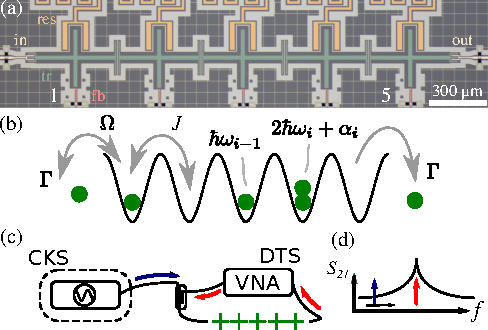
\includegraphics[width=1\linewidth]{Pictures/scheme.pdf}
	\caption{\textbf{(a)} Optical image of the device (false-colored). Input and output waveguides (beige) are strongly coupled to the edge transmons (green), which can be dispersively read out via auxiliary resonators (orange) and tuned via flux lines (red). \textbf{(b)} Interpretation of the device as a B-H lattice with five sites. Bosons are inserted from the left by a drive of strength $\Omega$, and can leak from both sides at rate $\Gamma$. The energy of a localized boson is $\hbar \omega$, and adding another boson to the same site costs $U = \hbar \alpha$. Excitations can tunnel back and forth between sites at rate $J$.}
	\label{fig:scheme}
\end{figure}

To obtain analytical predictions for the trasmission in the steady state, one can use the input-output formalism. Since we use classical drive, we assume that the input field mode amplitude is related to the drive strength via $\sqrt{\gamma_1} \langle  \hat b_{in}^\dag \rangle = i \Omega/2$, which follows from the quantum Langevin equations. The output field operator $\hat b_{out}^\dag \approx \sqrt{\gamma_5} \hat b_5^\dag$. From this, we obtain
\begin{equation}
	S_{21} = \frac{\langle \hat b_{out}^\dag \rangle}{\langle \hat b_{in}^\dag \rangle} = \frac{2\Gamma }{i\Omega} \Tr[\hat \rho_{ss} \hat b_5^\dag],
\end{equation}
where $\hat \rho_{ss}$ is calculated from $\mathcal L \rho_{ss} = 0$. Physically, this expression means that to observe some transmission, one must indirectly excite the rightmost transmon by irradiating the leftmost one. However, this is not an essentially quantum-mechanical effect. In the limit of $\alpha_i = 0,\ \forall i$ or, alternatively, $\Omega \ll \Gamma$, the system reduces to a chain of classical coupled oscillators. In the degenerate case when $\omega_i = \omega,\ \forall i$, it will produce transmission peaks at detunings $\delta = 0, \pm J, \pm \sqrt{3} J$ from $\omega$ (see Supplementary Materials). In the quantum-mechanical description, these frequencies remain in the spectrum due to the correspondence principle; however, new lines caused by purely quantum-mechanical processes are expected to appear.


\begin{figure}
	\centering
	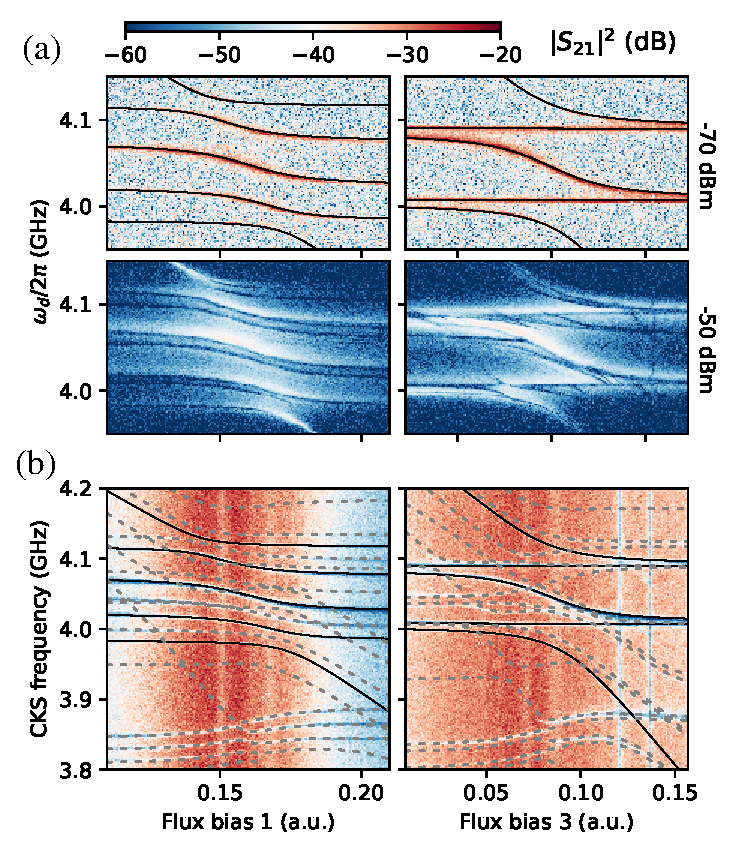
\includegraphics[width=1\linewidth]{Pictures/fig2}
	\caption{Transmission through the chain depending on the flux bias voltages 1 (left) and 3 (right) swept around the degeneracy point. In the top row, we show the fit (dashed lines) of the lowest five transitions of \autoref{eq:bose-hubbard} for $J/2\pi = 41$ MHz, $\omega_i/2\pi \approx 4.05$ GHz, coinciding with the classical normal modes solution. From top to bottom, as the microwave power is increased, we observe how the system transitions from the classical linear regime to the photon blockade regime.}
	\label{fig:transmission}
\end{figure}


\begin{figure}
	\centering
	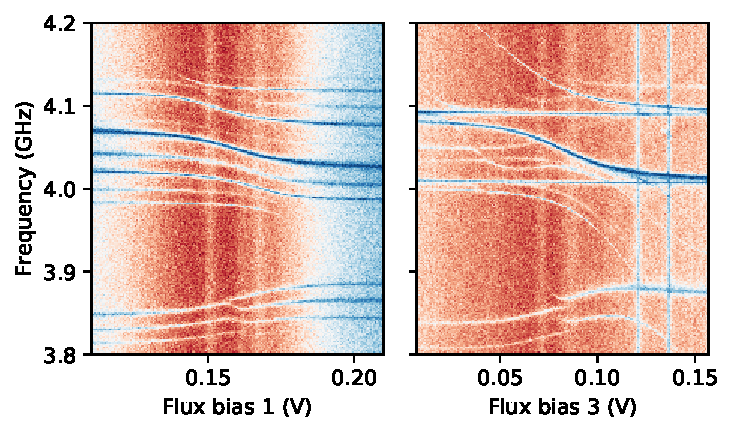
\includegraphics[width=1\linewidth]{Pictures/cktt}
	\caption{Cross-Kerr spectroscopy of the the third mode (the brightest spectral line) for two sweep configurations identical to \autoref{fig:transmission} showing the emergent band structure of the artificial crystal.}
	\label{fig:cktt}
\end{figure}

In \autoref{fig:transmission} we show the transmission through the system sweeping the frequency of one of the transmons while keeping the others degenerate at 4.05 GHz. Comparing the left and the right panels of \autoref{fig:transmission}, one may observe that the first transmon interacts with all normal modes, and the third one is decoupled from the even modes. This behaviour at single-photon power is consistent both with the classical coupled mode theory and the quantum-mechanical tight-binding description. However, when the incident power is increased, the behaviour of the system starts to change in a sharp contrast with classical linear theory whose predictions are power independent. At first, the peaks broaden, similar to the results observed previously \cite{astafiev2010resonance}. However, at even higher powers allowing multiphoton transitions, we find spectral manifestations of the many-body states of the system which do not have a classical analog and cannot be observed in a non-composite quantum system. We thus call this behaviour a classical-to-quantum transition with increasing power. The peculiar dark line structure in the lower right corner of \autoref{fig:transmission} implies the underlying complexity of the manybody eigenstates and eigenlevels and signifies the regime of chaotic behaviour of the classical Hamiltonian of the system \cite{zimmermann1986manifestation}.


\begin{figure*}
	\centering
	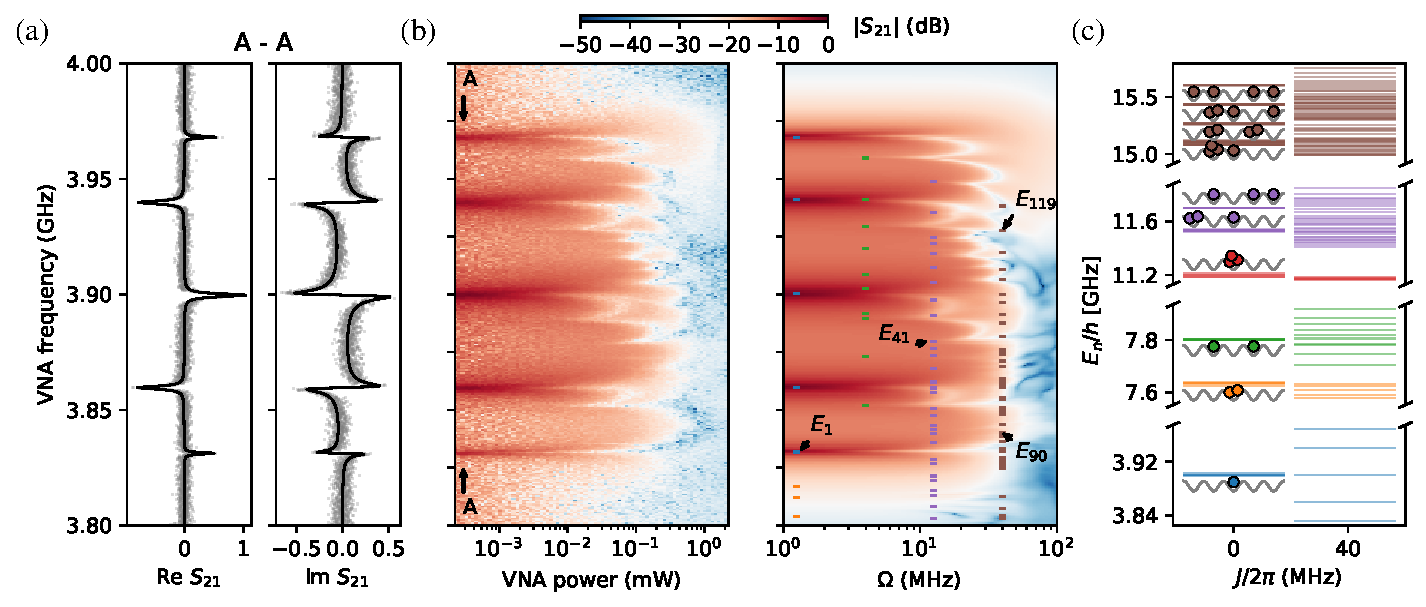
\includegraphics[width=0.9\linewidth]{Pictures/fig3}
	\caption{\textbf{(a)} The analytical solution for the $S_{21}$ in the linear regime (smooth curves) fitted to the low power data (clouds). Extracted values for the relaxation rates are [19.9,  1.2,  0.6,  1.0, 18.4] MHz. \textbf{(b)} Experimental and simulated $S_{21}$. The driving power is calibrated to match the corresponding Rabi frequency}
	\label{fig:cq_transition}
\end{figure*}

In \autoref{fig:cq_transition}, we show in greater detail this transition behaviour of the system when all five transmons are degenerate, $\omega_i/2\pi = 3.9$ GHz. The coupling to the transmission lines and internal dissipations can be estimated from the fit of the complex transmission coefficient predicted by the linear model (see Supplementary Materials) which is shown in \autoref{fig:cq_transition}. Additionally, we can estimate the overall attenuation in the measurement system and extract only the transmission through the chain. We find that the third mode has nearly unity transmission, as from \autoref{fig:transmission} it is only coupled to one ``bulk'' transmon, and thus has the least internal dissipation. Next, we we increse the power of the incident radiation and observe the multiphoton transitions to the higher energy bands. The experimental data agrees very well with the numerical steady-state simulation of the five three-level transmons. This method of measurement does not allow to see all transitions due to the selection rules. However, the increase of the density of states and their randomness is obvious. 





\bibliography{papers_bibliography}% Produces the bibliography via BibTeX.	
\end{document}